\documentclass[a4paper,11pt,dvipdfmx]{ujarticle}
% パッケージ
\usepackage{graphicx}
\usepackage{url}
% レイアウト指定を記述したファイルの読み込み
\input{layout}

% タイトルと氏名を変更せよ.
\title{日本におけるデジタル化の状況}
\author{G584752025 平松 駈}

\begin{document}

\maketitle %ここにタイトルが入る

% ここから本文
\section{デジタル競争力ランキング}
国際経営開発研究所(IMD)の調査\cite{oecd}によると,日本のデジタル競争ランキングは図\ref{fig:fig41}に示すように,
調査対象の64カ国中,総合で28位,技術分野で30位となっている.

% 本文(1)
%  参考文献の参照: \cite{}
%  図番号の参照: \ref{}
% を使う
% 文献データベースのキーワードは oecd と imd
% になっている.

% 図の挿入
\begin{figure}[htbp]
\centering
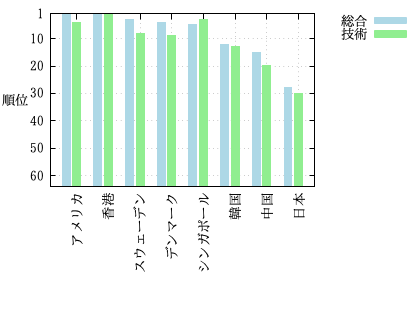
\includegraphics{fig41.png}
\caption{デジタル競争力ランキング(64カ国中)}\label{fig:fig41}

\end{figure}
% を
\begin{figure}[htbp]
\end{figure}
% で囲み
% \caption{}
% で図のタイトルを入れる.
% \label{}
% を使って図番号が参照できるようにする
% また,
% \centering
% で図が中央に来るようにする


\newpage



% 節見出し(2)
\section{ブロードバンドの整備状況}
% 本文(2)
OECDによるブロードバンド回線の普及に関する調査\cite{imd}によると,表\ref{tbl:mytbl}に示すように,
日本における100人あたりの光ファイバー回線の加入者数は29.0で,韓国,スウェーデン,ノルウェーに続いて第4位になっている.
% 表の挿入
\begin{table}[htbp]
    \centering
    \caption{光ファイバー回線の加入者数(100人あたり)}\label{tbl:mytbl}
    \begin{tabular}{c|c|c|c}
        \hline
        順位 & 国名 & 加入者数 \\
        \hline
        1位 & 韓国 & 38.2 \\
        \hline
        2位 & スウェーデン & 31.9 \\
        \hline
        3位 & ノルウェー & 29.5 \\
        \hline
        4位 & 日本 & 29.0 \\
        \hline
        5位 & アイスランド & 28.8 \\
        \hline
        6位 & スペイン & 27.3 \\
        \hline
        7位 & ポルトガル & 25.1 \\
        \hline
        8位 & ニュージーランド & 23.6 \\
        \hline
        9位 & リトアニア & 22.3 \\
        \hline
        10位 & フランス & 21.2 \\
    \end{tabular} 
\end{table}
% \begin{tabular}
% \end{tabular}    
% による表の記述を 
% \begin{table}[htbp]
% \end{table}
% で囲み
% \caption{}
% で表のタイトルを入れる.
% \label{}
% を使って表番号が参照できるようにする
% また,
% \centering
% で表が中央に来るようにする

% ーーー
% 見出し(3)
\section{考察}
\begin{itemize}
    \item シンガポールのみ総合順位よりも技術分野順位が高い
    \item いずれの国も総合順位と技術分野順位の差が10位以内になっている
\end{itemize}
% 考察
%
% \begin{itemize}
% \end{itemize}
% を使って箇条書きで記述する

% ここに参考文献が入る
%
\bibliographystyle{junsrt}
\bibliography{exercise.bib}

\end{document}